\chapter{State of the Art} \label{chap:sota} \minitoc

A data stream has a temporal dimension and the underlying process that generates data can change over time \cite{Aggarwal-Evolving-Data-Streams, Domingos-Mining-Time-Data-Streams}. In this chapter, we discuss the most relevant work for the problem of detecting data pattern shifts in real-time over true sliding windows using resource-lightweight approaches on streaming systems, presented in Chapter \ref{chap:intro}. We present a wide analysis of several categories of algorithms to be able to identify what's the region of this vast landscape of methods that may be useful to build the desired system. 

\section{Outlier Detection in Time-Series Data} \label{sec:outliers}
Blázquez-García \emph{et al.} review state of the art outlier detection techniques and present a taxonomy based on the main aspects of outlier detection methods \cite{Blazquez-Garcia-Review-Anomaly-Detection}. From multiple reviews on these kind of methods \cite{Aggarwal-Outlier-survey, Aguinis-Outlier-survey, Chandola-Outlier-survey-2009, Hodge-Outlier-survey, Xu-outlier-survey-2019} we chose to adopt the taxonomy presented by Blázquez-García \emph{et al.} due to its focus on time-series data.

In this work, the authors define a time-series as a collection of data points sorted by time; and outliers as observations that do not follow the expected behavior. This definition is similar to the concept of outlier provided by Hawkins in 1980 where he states that an outlier is “an observation which deviates so much from other observations as to arouse suspicions that it was
generated by a different mechanism" \cite{Hawkins-Outliers}. Furthermore, Blázquez-García \emph{et al.} allude to the fact that outliers are often referred to in the literature as \textit{"anomalies, discordant observations, discords, exceptions, aberrations, surprises, peculiarities or contaminants"} which for the purpose of their review and this thesis all refer to outliers. In summary, outlier detection refers to the process of finding anomalies in data. An anomaly (or outlier) relates to a point in time where the behavior of the system does not match the expected one. Note that under this definition the presence of outliers or anomalies does not necessarily imply a problem. 

The authors evaluate an outlier detection method on three different axes: the input data type, the outlier type to detect and the uni or multivariate nature of the method. Figure \ref{fig:outlier-taxonomy} presented by the authors in \cite{Blazquez-Garcia-Review-Anomaly-Detection} summarizes these categories.

\begin{figure}[!htb]
  \begin{center}
    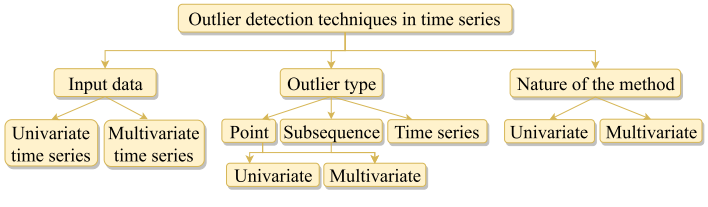
\includegraphics[scale=0.55]{figures/outlier-method-taxonomy.png}
    \caption{Outlier detection method taxonomy}
    \label{fig:outlier-taxonomy}
  \end{center}
\end{figure}

The \textit{input data} axis refers to the type of time-series the method uses as input. According to this criterion, an outlier detection method is said to work with a univariate time-series or a multivariate one. A univariate time-series refers to a time-series consisting of a list of values generated by a single time-dependent variable throughout time. On the other hand, a multivariate time-series has more than one time-dependent variable. Most importantly, each variable is not only time-dependent but may also have dependencies on other variables. 

The \textit{nature of the method} axis refers to the type of analysis performed by the outlier detection method. An outlier detection method may perform a univariate or multivariate analysis. A multivariate analysis considers all variables in the time-series simultaneously while univariate analysis looks at each variable independently. An outlier detection method can take as input a multivariate time-series but perform a univariate analysis, one per time-series of the multivariate input. On the other hand, to perform multivariate analysis, the input data type must be multivariate as well.

The third and final axis is the \textit{outlier type} the method aims to report. The authors identify three distinct outlier types: point outliers, subsequence outliers and time-series outliers. A point outlier corresponds to a single data point in time that deviates from the expected value. These point outliers can be uni or multivariate, depending on the nature of the method. A univariate point outlier is a single time-dependent variable that stands out from the rest of the time-series. On the other hand, a multivariate point outlier takes into account multiple time-dependent variables in comparison to the remaining time-series. Subsequence outliers refer to a sequence of points in time that together show anomalous behavior, but may not be individually considered outliers. Similarly to point outliers, a subsequence outlier may take into account a single time-dependent variable or multiple ones. The authors classify them as univariate subsequence outliers and multivariate subsequence outliers, respectively. Lastly, time-series outliers refer to entire time-series being outliers themselves. This type of outliers can only be detected if the input data is multivariate, to be able to compare multiple time-series.

\subsection{Univariate Point Outlier Detection}

Univariate point outlier detection methods are further broken down into three categories: model-based, density-based and histogram-based (Figure \ref{fig:point-outlier-taxonomy}) .
\begin{figure}[!htb]
  \begin{center}
    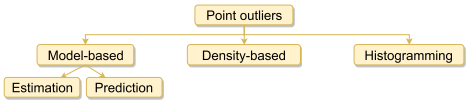
\includegraphics[scale=1]{figures/taxonomy-point-outlier-uni.png}
    \caption[Point outlier detection in univariate time-series taxonomy]{Point outlier detection in univariate time-series taxonomy \cite{Blazquez-Garcia-Review-Anomaly-Detection}}
    \label{fig:point-outlier-taxonomy}
  \end{center}
\end{figure}

The univariate point outlier detection methods based on models are the most common. For each timestamp of the time-series, the models compute the predicted value for the time-dependent variable and compare it with the observed value. If the difference between the predicted value and the observed one is above a certain threshold the data point at the current timestamp is considered an outlier. Mathematically, given the predicted value $p\textsubscript{t}$, the actually observed value $x\textsubscript{t}$ and the user-defined threshold $\alpha$, $x\textsubscript{t}$ is considered an outlier at timestamp \textit{t} if and only if:
\begin{equation*}
    |x\textsubscript{t}-p\textsubscript{t}|>\alpha
\end{equation*}
Model-based point outlier detection methods can be one of two types: estimation or prediction models. The main difference is that estimation model-based methods use past and future data while prediction model-based methods use only past data and infer current and future values. Because of this, prediction model-based outlier detection methods can be used in real-time to process streaming time-series, while estimation based methods can only be used in batch.

Density-based univariate point outlier detection methods rely on the clustering of data points and neighbor counting. For example, nearest neighbor based methods consider a datum an outlier if it has less than $k$ neighbors. Distance between two points is usually measured using the Euclidean distance \cite{elementary-algebra}. Two points are said to be neighbors if they are close to each other --- \textit{i.e.}, the distance between them is less than or equal to a given threshold $\alpha$.

The authors provide little detail on the last category, the histogram-based one. The authors state that these methods are ``based on detecting the points whose removal from the univariate time series results in a histogram representation with lower error than the original''.

\subsubsection{Neighbor-Based Pattern Detection for Windows Over Streaming Data} \label{alg:extran}
 
Yang \emph{et al.} propose \emph{Extra-N} \cite{Yang-Neighbor-Based-Pattern-Detection}, a method for incremental detection of point outliers in sliding window scenarios. Data points are considered outliers if they have few neighbors, \textit{i.e.}, less than a user-defined threshold $\alpha$ of neighbors within a user-defined range $\theta$. Figure \ref{fig:point-outlier} depicts points plotted in their feature space (in this case only two dimensions or features are used, x1 and x2) and a point outlier for $alpha=2$ points and any given $\theta$.
\begin{figure}[!htb]
  \begin{center}
    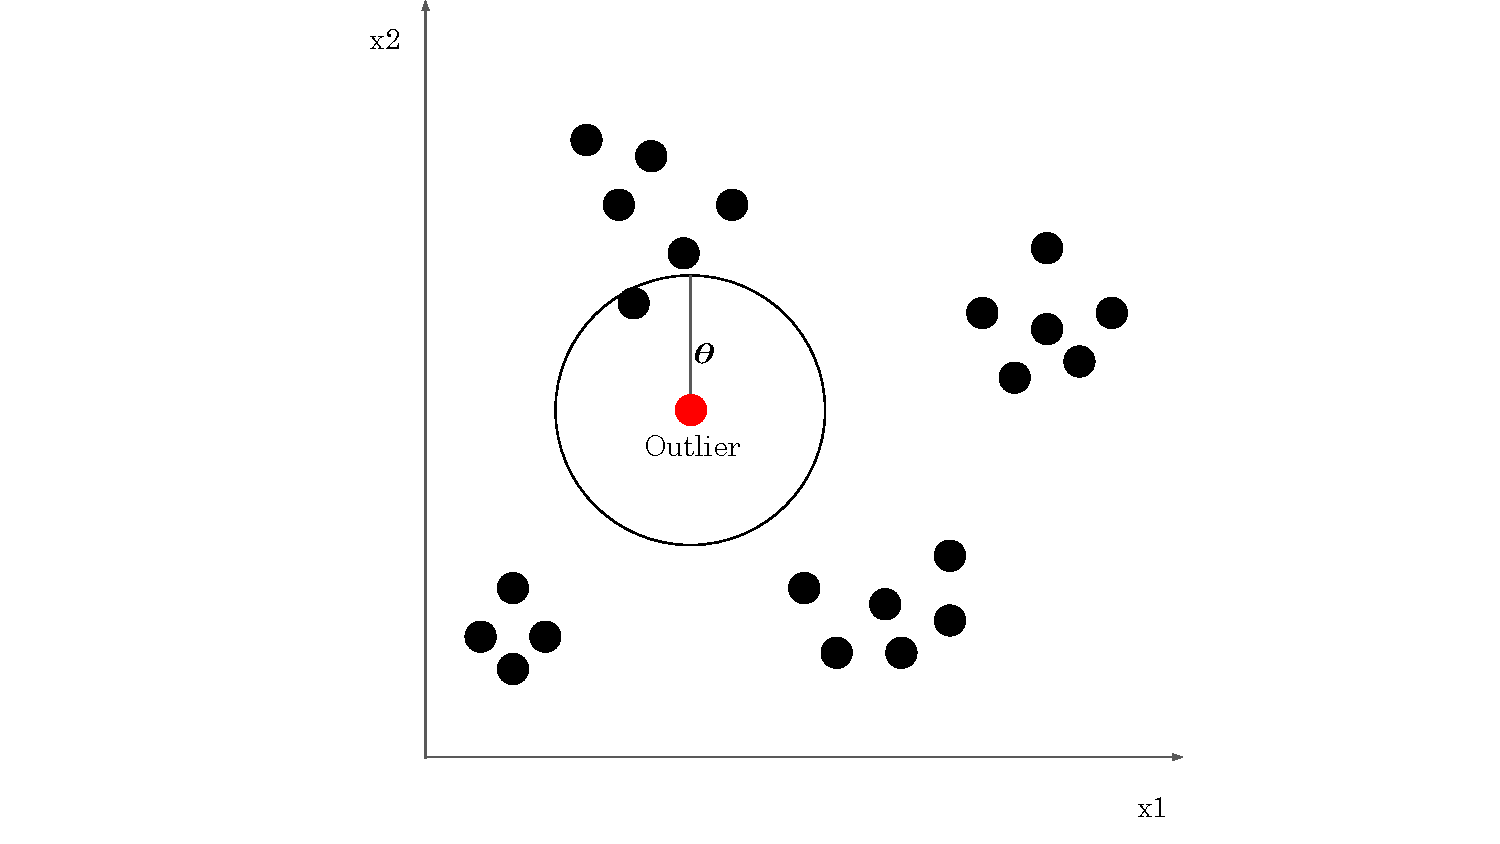
\includegraphics[scale=0.6]{figures/point-outlier.pdf}
    \caption[Density-based point outlier]{Density-based point outlier for $\alpha=2$ and a given $\theta$}
    \label{fig:point-outlier}
  \end{center}
\end{figure}

The key idea is to predict the expiration of any data point in the sliding window and pre-handle the impact it has on its neighbors. The authors introduce the concept of \emph{lifetime neighbor counts} or \textit{lt\_cnt}. The \textit{lt\_cnt} of a data point corresponds to a sequence of predicted neighbor counts, \textit{i.e.}, the number of predicted neighbors a data point has in any future window where it exists. More precisely, each entry on \textit{lt\_cnt} records the number of neighbors that are known to survive in future windows. 

For example, consider a window \textit{W\textsubscript{0}} and a data point \textit{p\textsubscript{0}} with three neighbors: \textit{p\textsubscript{1}}, \textit{p\textsubscript{2}} and \textit{p\textsubscript{3}}. Assume \textit{p\textsubscript{1}} expires after \textit{W\textsubscript{0}}, \textit{p\textsubscript{2}} and \textit{p\textsubscript{3}} expire after \textit{W\textsubscript{1}} and \textit{p\textsubscript{0}} expires after \textit{W\textsubscript{2}}. This implies that at \textit{W\textsubscript{0}}, 
\[ p\textsubscript{0}.lt\_cnt = \{W\textsubscript{0}: 3, W\textsubscript{1}: 2, W\textsubscript{2}: 0\} \]
The lifetime neighbor counts (\textit{lt\_cnt}) carry enough information to compute density-based point outliers: for each data point check if the first or current element of \textit{lt\_cnt} is less than a user-defined threshold $\alpha$ to decide whether that data point is an outlier or not.


\subsubsection*{Method classification}
Extra-N can take both uni or multivariate time-series as input data. However, it does not relate multiple time-series and it does not take into account possible dependencies between different time-dependent variables. In that sense, and according to the presented taxonomy (Figure \ref{fig:outlier-taxonomy}), the method accepts uni or multivariate time-series as input but is of univariate nature. Last but not least, Extra-N aims to detect univariate point outliers. These point outliers are identified based on the density of the region or neighborhood they belong too. Hence, we say Extra-N is a density-based univariate point outlier detection method (Figure \ref{fig:point-outlier-taxonomy}).

\subsubsection*{Time complexity}

To find outliers, Extra-N has to do a linear search through the list of points and check the neighbor counts. Hence, for outlier detection, this method shows \textit{O(n)} complexity with \textit{n} as the number of points. Additionally, for each new data point \textit{p\textsubscript{i}}, Extra-N has to perform a range query search centered on it to find its neighbors and increment their lifetime neighbor counts by one. The runtime complexity of a range query search is \textit{O(log(n))} \cite{range-query-log} with \textit{n} as the number of data points.

In summary, Extra-N shows logarithmic time complexity when updating the sliding window and linear time complexity when looking for outliers, both relative to the window size.


\subsubsection*{Space complexity}
Extra-N has to keep a lifetime neighbor count dictionary-like object for each window data point. For that reason, Extra-N achieves linear memory consumption relative to the number of data points in the window.

\subsubsection*{Applicability to our Hypothesis}
Extra-N memory consumption grows linearly in regards to window size, so it does not fit our desired lightweight system architecture. Furthermore, updating the sliding window should be done in constant time, which is not the case for Extra-N. Hence, we will not use this algorithm.

\subsubsection{Real-Time Stream Anomaly Detection with Hierarchical Temporal Memory}
Ahmad \& Purdy present an anomaly detection technique based on an online algorithm called Hierarchical Temporal Memory (HTM)\footnote{https://github.com/numenta/nupic} \cite{Ahmad-HTM}. HTM has a few properties that are desirable for data stream anomaly detection scenarios. First, it is an unsupervised algorithm that requires no labels. This property comes in handy when monitoring a data stream in real-time, where labels for incoming data will likely be absent. Additionally, HTM adapts to noisy domains. In other words, random variations in the underlying distribution of incoming data that do not persist throughout time will be ignored. Furthermore, HTM detects both spatial and temporal anomalies --- \textit{i.e.}, changes in magnitudes of data or unusual timing for particular patterns, respectively.   

HTM is an online learning algorithm, meaning that it adapts to changing statistics of the underlying data stream. In other words, if there is a sudden abrupt change in the distribution of a specific time-dependent variable, the algorithm will raise an alert. However, if an initial spike that was assumed to be an anomaly becomes frequent, then the algorithm adapts and assimilates this as "a new reality" and stops classifying it as anomalous. Unfortunately, this property is not desirable in our system. Our stream monitoring system must report changes relatively to an initial static configuration (reference or normality period) and should not accept a new distribution as the new standard.

\subsubsection*{Method classification}
Similarly to Extra-N presented in Section \ref{alg:extran}, the Hierarchical Temporal Memory (HTM) algorithm accepts both uni and multivariate time-series as input data but does not perform a multivariate analysis. Hence, we say it accepts both uni and multivariate inputs but is univariate in nature. HTM focuses on finding point outliers, but unlike Extra-N, which is density-based, HTM is a model-based approach. Specifically, HTM is a prediction model-based approach for univariate point outlier detection (Figures \ref{fig:outlier-taxonomy} and \ref{fig:point-outlier-taxonomy}).


\subsubsection*{Applicability to our Hypothesis}
Online learning algorithms that adapt to data pattern shifts and eventually consider them regular patterns are not viable to our goals. We need a monitoring system that alerts data pattern shifts continuously until they match the initial configuration again. Additionally, insights produced by machine learning models are not human-understandable, leaving the user confused about why an anomaly report was made. In conclusion, we do not deem HTM applicable to our solution.


\subsubsection{DeepAnT}
Munir \emph{et al.} present DeepAnT, a deep learning-based approach for the detection of anomalies in time-series data \cite{Munir-DeepAnT}. DeepAnT uses unlabeled data to capture and learn the distribution of the data stream used to forecast the normal behavior of the time-series. This method is unsupervised - \textit{i.e.}, it requires no labels - which is an advantage in a streaming scenario where real-time decisions have to be made before labels are effectively-known. It is capable of detecting point anomalies in time series data with periodic and seasonal characteristics.

DeepAnT employs a Convolutional Neural Network (CNN) as its time-series predictor module. Before monitoring a data stream, the CNN model must be trained. The model can be trained with a small dataset while achieving good generalization capabilities due to the effective parameter sharing of the CNN. Additionally, the dataset used to train the model does not require labels.

\subsubsection*{Method classification}
DeepAnT takes as input a uni or multivariate time-series but is a univariate method by nature --- \textit{i.e.}, it does not find correlations between multiple time-dependent variables. The model used by DeepAnT is a Convolutional Neural Network (CNN), used to make predictions on the future time-series values and measure differences with the actual observed values. Hence, DeepAnT is a prediction model-based univariate point outlier detection method (Figures \ref{fig:outlier-taxonomy} and \ref{fig:point-outlier-taxonomy}).

\subsubsection*{Applicability to our Hypothesis}
Similar to the HTM algorithm presented, DeepAnT adapts to the underlying distribution of the data stream. In other words, if the data patterns shift from the initial configuration but stabilize, DeepAnT will accept it as it is. As mentioned, our goal is to build a monitoring system that alerts data pattern shifts continuously, until they match the initial configuration again.

\subsection{Univariate Subsequence Outlier Detection} \label{sec:uni-sub-out}
Similarly to point outlier detection methods, Blázquez-García \emph{et al.} \cite{Blazquez-Garcia-Review-Anomaly-Detection} split subsequence outlier detection methods into uni and multivariate ones (Figure \ref{fig:outlier-taxonomy}). Furthermore, the authors split univariate subsequence outlier detection methods into five different axes as seen in Figure \ref{fig:subsequence-outlier-taxonomy}.

\begin{figure}[!htb]
  \begin{center}
    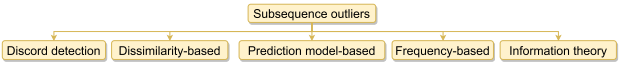
\includegraphics[scale=0.8]{figures/taxonomy-subsequence-outlier-uni.png}
    \caption[Subsequence outlier detection in univariate time-series taxonomy]{Subsequence outlier detection in univariate time-series taxonomy \cite{Blazquez-Garcia-Review-Anomaly-Detection}}
    \label{fig:subsequence-outlier-taxonomy}
  \end{center}
\end{figure}

Methods in the discord detection category compare each subsequence in the time-series with the other subsequences within the time-series to find out the most unusual ones. Each subsequence is compared to the others using a distance metric, for instance, the Euclidean distance. The brute-force way of accomplishing this requires a pairwise comparison of all the subsequences, effectively resulting in quadratic time complexity. These methods find the most unusual subsequence in a time-series. However, as the authors put it, these methods lack a reference or normality state and hence do not accurately report outliers.

On the other hand, univariate subsequence outlier detection methods based on dissimilarity are identical to the previous discord detection based methods but use a reference of normality. The representations used for the subsequences and the reference of normality vary among methods in this class of outlier detection methods but they are based on comparison of the reference or normality subsequence with the ones being analyzed for outlier detection. Once again, the metric used to measure the distance between the reference period subsequence and the other ones depends entirely on the method and subsequence aggregation or representation. Finally, when the measured distance is above a certain threshold, these methods classify the subsequence as an outlier or an anomaly.

Prediction model-based univariate subsequence outlier detection methods assume that the reference or normality period is composed of past events. Similarly to univariate point outlier detection methods based on prediction models, these models train on past data and make predictions of the future. Subsequences that deviate from the model's prediction are classified as outliers.

Frequency-based univariate subsequence outlier detection methods also use a reference period and compute the frequency of each subsequence in the reference or normality period. Hence, a subsequence will be an outlier if it does not appear as frequently as expected in subsequent periods.

Lastly, we have information theory based methods for univariate subsequence outlier detection, which according to the authors \textit{"are closely related to the frequency-based methods"}. This type of method not only measures the frequency of subsequences but relates it with the information carried by the subsequence. Mathematically, a subsequence $S$ will be an outlier if

\begin{equation*}
    I(S) \times F(S) > \alpha
\end{equation*}

with $F(S)$ as the frequency of subsequence $S$, $I(S)$ as the information carried by $S$ and $\alpha$ as a given threshold. According to the authors, \textit{"I(S) is computed taking into account the number of times the symbols within S are repeated through the series"}. The authors explain that if \textit{F(S)} is large --- \textit{i.e.}, S occurs frequently --- then \textit{I(S)} will be closer to 0.

\subsubsection{A two window paradigm algorithm for change detection} \label{kifer}
Kifer \emph{et al.} propose that detecting change in data streams can be reduced to testing if two windows have different underlying distributions \cite{Kifer-Detecting-Change}. The proposed method uses two windows, a reference \textit{W\textsubscript{1}} and a sliding one \textit{W\textsubscript{2}}. Both windows are tuple-based, have size \textit{k} and the sliding window is a true sliding one (recall Section \ref{sec:windows} and the expression \ref{math:windows}). The reference window \textit{W\textsubscript{2}} works as a \textit{reference of normality} and contains the first \textit{k} points of the stream that occurred after the last detected change.

The algorithm begins by filling both windows with the first \textit{k} tuples. Then it slides window \textit{W\textsubscript{2}} by one tuple, since it is a true sliding window, for each incoming event from the data stream. In between slides, the algorithm checks for change by applying a distance function \textit{d} taking as input both the reference and the sliding windows, which measures the discrepancy between both. Whenever this distance is above a certain threshold $\alpha$, the algorithm raises an alert. After raising an alert, both windows are re-initialized with the next \textit{k} items.

Note that after a change is detected, the reference window is updated with the next \textit{k} tuples from the stream. As we have stated, we want a method that does not adapt to the data stream changes and instead keeps raising alerts until the sliding window data distribution returns to the one seen in the reference period. It is trivial to adapt this method to always use the same reference period. To do so, we simply keep the original reference window and do not update it after each alert.

This algorithm reduces change detection in data streams to testing whether two samples --- \textit{reference} and \textit{sliding} windows --- are generated by different distributions. The authors study methods for identifying differences in distribution between two samples and implement them as the \textit{d} function. They provide as examples of a possible \textit{d} function implementation the  Kolmogorov–Smirnov Test \cite{Kolmogorov-Smirnov} and the Wilcoxon-Signed-Rank Test \cite{Wilcoxon}.

\subsubsection*{Method classification}
The method devised by Kifer \emph{et al.} can take uni or multivariate input (if we use one pair of reference/target windows for each time-series) but performs a univariate analysis as it does not find correlations between time-dependent variables. This two-windowed method measures the difference between both windows, the reference and the sliding one. Furthermore, instead of detecting point outliers, the alerts produced indicate the entire window (or subsequence) shows anomalous behavior. Hence, according to the taxonomy presented in Figure \ref{fig:subsequence-outlier-taxonomy}, this method is a dissimilarity-based univariate subsequence outlier detection method.

\subsubsection*{Time complexity}
The authors show that it is possible to compute the distance between both windows in logarithmic time regarding window size \textit{k}. Because the entire sliding window is held in memory, a window update is tantamount to removing the head of the list (element eviction) or appending a new element to the tail (element insertion), which is done in constant time. Thus, for each new event, the method evicts the oldest element, inserts the new one and computes the distance between the reference and sliding windows. In big O notation, the largest and determining factor is the computation of the distance function, done in \textit{O(log(k))} time, with \textit{k} as the size of both windows.

\subsubsection*{Space complexity}
The method makes use of two \textit{k}-sized windows, thus storing \textit{2k} elements. Hence, memory consumption grows linearly with window size.

\subsubsection*{Applicability to our Hypothesis}
In this thesis, we want to detect and alert data pattern shifts with a low memory footprint. The method proposed by Kifer \emph{et al.} grows linearly with window size, making it unfit for large windows, our use case.

However, this two-window paradigm encodes a static normal or reference period in one window and the observed streaming values in a sliding one. Since in this thesis we want to report streaming data pattern shifts relatively to a reference period, we use a similar two-windowed model, but use lightweight and incrementally maintainable aggregations over both windows.


\subsubsection{SAMM: Automatic Model Monitoring for Data Streams}

Sampaio \emph{et al.} present SAMM \cite{SAMM}, an automatic model monitoring system for data streams. Similarly to the method presented in Section \ref{kifer}, SAMM uses two windows: the reference window R and the target window T. Window T contains the last $n_t$ elements and window R the $n_r$ elements of a reference period, which is prior to T. SAMM has two main components that interest us: the one responsible for computing the signal and the one that defines the signal threshold. 

The Machine Learning (ML) model being monitored outputs a series of scores for each transaction. The authors build two histograms: one with the model scores for the reference window R and another for the target window T. The signal is a measure of similarity between both histograms $H_R$ and $H_T$. The authors considered using the Kolmogorov-Smirnov \cite{KolomogorovSmirnov, Kolmogorov-Smirnov}, Kuiper \cite{KuiperTest} and Anderson-Darling \cite{AndersonDarling} test but ultimately used the Jensen-Shannon Divergence (JSD) \cite{JSD} to measure the similarity between both histograms. The JSD outputs a value between 0 and 1, with totally different histograms being assigned a value of 1. The signal is then computed by applying the JSD metric to both histograms $H_R$ and $H_T$ at each new event.

To compute the threshold for the JSD signal, the authors maintain a histogram of observed JSD values during streaming. To efficiently maintain the JSD histogram, they devise an algorithm called SPEAR which stands for Streaming Percentiles EstimAtoR. SPEAR is linear in time and space complexity regarding the number of histogram bins, which is a small and fixed constant. This way, for a new JSD value measured between the histogram $H_R$ and histogram $H_T$, they compare it with the histogram and alert if above a certain percentile (\textit{e.g.}, the 99th percentile).

\subsubsection*{Method classification}
SAMM can take uni or multivariate time-series as input but performs a univariate analysis. This method is also a two-windowed method that measures the difference between reference and target sliding windows. The alerts produced report the entire target window as anomalous. According to the taxonomy presented in Figure \ref{fig:subsequence-outlier-taxonomy}, we classify this method as a dissimilarity-based univariate subsequence outlier detection method.

\subsubsection*{Time complexity}
For each new event, SAMM updates the target window T, updates the target histogram $H_T$, computes the JSD between $H_T$ and $H_R$, checks if this value is above a certain percentile and finally updates the histogram of JSDs with the new one. 

Maintaining the target window, \textit{i.e.}, evicting old events and inserting new ones, updating the target histogram $H_T$, computing the JSD between $H_T$ and $H_R$ and checking if it is above a given percentile are all done in constant time. Updating the JSD histogram and dynamically resizing the bins with the SPEAR algorithm takes $O(n)$ time with $n$ as the number of bins. Because the number of bins is small and constant, the update of the JSD histogram is also done in constant time.

Overall, SAMM can process each event in constant time and is suitable for data stream monitoring.

\subsubsection*{Space complexity}
SAMM keeps in memory a reference window, a target window, a reference histogram, a target histogram and a JSD histogram. The histograms can have a small and fixed number of bins so they are not the dominant factor contributing to SAMM's space complexity. Instead, because SAMM keeps two windows in memory, it stores all the events belonging to them. Assuming $n_t$ as the size of target window and $n_r$ as the size of the reference window, SAMM has $O(n_r + n_t)$ space complexity.

\subsubsection*{Applicability to our Hypothesis}
SAMM was designed to work for small-time periods. Hence, for the authors, keeping the reference and target windows in memory was no issue. However, in our solution, we need sublinear time and space complexities to handle large windows of data. This implies we can not directly use SAMM to solve our problem.

However, SAMM has interesting properties we can use in our final solution. First, SAMM also uses a two-window paradigm: a reference and a target sliding one. This is similar to the method seen in Section \ref{kifer}, which may indicate this is a valid and tested approach to follow. Additionally, SAMM aggregates the contents of both windows as histograms and utilizes a statistical divergence test, the Jensen-Shannon Divergence, to measure the similarity (or dissimilarity) between both. This gives them a measure of divergence which they use to raise alerts, which is another great idea to test. Finally, and contrarily to the previous method (Section \ref{kifer}), SAMM does not simply threshold this divergence value: it builds a distribution of divergence values and measures percentiles for new event's divergence values. This allows a user to easier define a threshold: instead of specifying a threshold between 0 and 1 for the JSD value, the user defines only a probability value, \textit{e.g.}, alert when the probability for a JSD value is equal or less than 1\% (percentile 99th).

Even though SAMM is not directly applicable in our context, it provides us with valid and promising ideas to test.


\section{Sliding Window Aggregation Algorithms} \label{sec:sota-swag-algs}

As discussed in Section \ref{sec:back-swag-algs}, a sliding window aggregation algorithm allows the computation of an exact or approximate aggregation over a sliding window. We want to find an aggregation that is suitable to encode our reference and streaming periods so we avoid keeping the entire sliding window in memory. Furthermore, we need an efficient algorithm to incrementally maintain this aggregation. We have presented Recalculate-From-Scratch (RFS) and Subtract-On-Evict (SOE) as the two most basic generic stream processing algorithms. In this section, we analyze other more sophisticated SWAG algorithms that fit different use cases, restraining the set of computable aggregations to certain families, as defined in Table \ref{tbl:aggregations-properties}.

\subsection{Two-Stacks} \label{sec:2stacks}
The Two-Stacks SWAG algorithm works for \textit{associative} aggregations (recall Table \ref{tbl:aggregations-properties}) in scenarios where the sliding window has First-In First-Out (FIFO) semantics --- \textit{i.e.}, elements are evicted in the same order they were inserted. Two-Stacks \cite{Tangwongsan-DABA} implements the FIFO queue using two stacks, namely the front stack F and the back stack B. Each element in each of the stacks is a pair \textit{<val, agg>} where \textit{val} is the item's value and \textit{agg} is the aggregation value of everything below it on the stack. The pseudocode for Two-Stacks can be seen in Algorithm \ref{pseudo:2-stacks}, assuming all functions have access to stacks F and B, with $\oplus$ as the \textit{combine} function and $\overline{\theta}$ as the identity value of the \textit{combine} function, such that $\overline{\theta} \oplus x$ = $x \oplus \overline{\theta}$ = x. For example, if $\oplus$ is the arithmetic sum then $\overline{\theta}$ is 0. If $\oplus$ is the arithmetic multiplication then $\overline{\theta}$ is 1.

Insertion of a new item is always made on stack B. The updated aggregation state is computed using the \textit{combine} function $\oplus$ taking as arguments the aggregation value \textit{agg} of the top element of stack B and the item's value \textit{val}. The pair pushed onto stack B is a pair with \textit{val} and the new aggregation value $\textit{agg} \oplus \textit{val}$.

Evictions correspond to a simple pop from stack F. However, when F is empty, the elements from stack B are flipped onto stack F, re-applying $\oplus$ to make sure each element in F holds the aggregation value of everything below in the stack. Given \textit{n} as the size of stack B, the occasional flip operation takes \textit{O(n)} time.

Computing the sliding window aggregation is done by applying the \textit{combine} function $\oplus$ to the aggregation values of each of the stacks' top element. 

\begin{algorithm}
    \caption[Two-Stacks]{Two-Stacks insert, evict and query methods}
    \label{pseudo:2-stacks}
    \begin{algorithmic}[1]
        \Function{getStackAggregationValue}{stack}
         \If{stack.isEmpty()} 
            \State \Return{$\overline{\theta}$} 
        \Else 
            \State \Return{stack.top().agg} 
        \EndIf
        \EndFunction
        
        \Function{query}{}
            \State \Return{getStackAggregationValue(F) $\oplus$ getStackAggregationValue(B)}
        \EndFunction
        
        
        \Function{insert}{v}
            \State{B.push( \{val: v, agg: getStackAggregationValue(B) $\oplus$ v\} }
        \EndFunction
        
        
        \Function{evict}{}
            \If{F.isEmpty()} \Comment{// Flip B onto F and update top aggregation value}
                \While {\textbf{not} B.isEmpty()}
                    \State{F.push( \{val: B.top().val, agg: B.top().val $\oplus$ getStackAggregationValue(F) \})}
                    \State{B.pop()}
                \EndWhile
            \EndIf
            \State{F.pop()}
        \EndFunction
    \end{algorithmic}
\end{algorithm}

\subsubsection*{Time complexity analysis}
Querying the aggregation state of the window and inserting a new element can be performed in constant time. However, while evicting an item is usually done in constant time, occasionally, a flip operation is required, consuming \textit{O(n)} time, with \textit{n} as the size of stack B. Because this flip is occasionally performed, the time complexity of Two-Stacks is said to be \textit{amortized} constant.

\subsubsection*{Space complexity analysis}
Two-Stacks uses two stacks as auxiliary data structures. The combined size of both stacks is at most the size of the sliding window \textit{n}. Hence, Two-Stacks has linear space complexity \textit{O(n)}.

\subsubsection*{Applicability to our Hypothesis}
Two-Stacks is a general sliding window aggregation algorithm to compute \textit{associative} aggregations. However, it is linear in space and occasionally performs the computationally intensive operation of flipping stack B onto stack F, making it unfit for our use case.


\subsection{De-Amortized Banker’s Aggregator} \label{sec:daba}

The De-Amortized Banker’s Aggregator (DABA) \cite{Tangwongsan-DABA} is a SWAG algorithm that allows the computation of \textit{associative} aggregations. This method carefully handles expensive operations and spreads them along the execution. As a result, the authors are able to turn the average-case behavior into worst-case behavior. This is commonly known as \textit{de-amortization}, hence the name. The main idea behind DABA's design is to avoid occasional expensive operations --- such as the flip operation in Two-Stacks --- by gradually executing them throughout runtime.

\subsection*{Data Structure}

DABA uses two queues, \textit{vals} and \textit{aggs}, both of size \textit{n}, seen in Figure \ref{fig:daba-ds}, which was directly taken from \textit{"Low-Latency Sliding-Window Aggregation in Worst-Case Constant Time"} by Tangwongsan \emph{et al.} Both queues share six pointers --- \textit{F, L, R, A, B} and \textit{E} --- which point to the same position for each queue. These pointers are always ordered as follows: $F \leq L \leq R \leq A \leq B \leq E$.

\begin{figure}[!htb]
    \begin{center}
      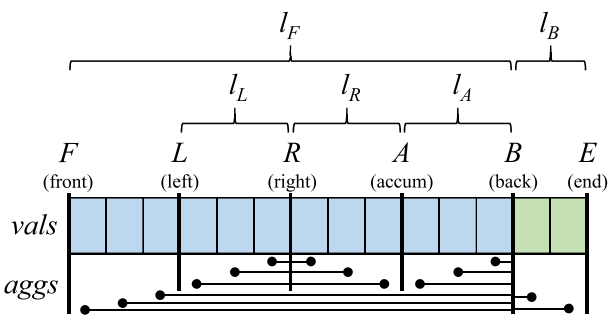
\includegraphics[scale=0.6]{figures/daba-ds.png}
      \caption[DABA data structure]{DABA data structure \cite{Tangwongsan-DABA}}
      \label{fig:daba-ds}
    \end{center}
\end{figure}

Queue \textit{vals} holds the actual sliding window contents. New values are pushed in the back and old values are popped from the front of the queue. Queue \textit{aggs} stores aggregations of sub-ranges of \textit{vals}. Aside from pointer \textit{E}, each pointer defines a sub-list and each sub-list is aggregated either to the left \textbullet--- or to the right ---\textbullet. If a sub-list is aggregated to the left \textbullet---, each \textit{aggs} element will be the aggregation value of all elements in \textit{vals} from that position to the right. On the other hand, if a sub-list is aggregated to the right ---\textbullet, each \textit{aggs} element will be the aggregation value of all elements in \textit{vals} from that position to the left. Values from \textit{vals} can be aggregated to the left or to the right because DABA restricts the aggregation to be \textit{associative} (refer to Table \ref{tbl:aggregations-properties}).

Figure \ref{fig:daba-ds} shows sub-lists \textit{l\textsubscript{F}}, \textit{l\textsubscript{B}}, \textit{l\textsubscript{L}}, \textit{l\textsubscript{R}} and \textit{l\textsubscript{A}}. Sub-list \textit{l\textsubscript{F}} is aggregated to the left for easier eviction. After an element is evicted, the new head of the queue \textit{aggs} --- pointed by \textit{F} --- already contains the aggregation value of all elements from \textit{vals} to its right side. Hence, evicting an element amounts to evicting from both \textit{vals} and \textit{aggs} queue. Similarly, \textit{l\textsubscript{B}} is aggregated to the right to facilitate insertion. Sub-lists \textit{l\textsubscript{L}}, \textit{l\textsubscript{R}} and \textit{l\textsubscript{A}} allow for incremental reversal of the right-aggregated \textit{l\textsubscript{B}} to the left-aggregated \textit{l\textsubscript{F}}. This incremental reversal is tantamount to adjusting pointers that causes shifts in sub-list boundaries. Thus, elements of \textit{aggs} may change from one sub-list to another and need to have its aggregation value recomputed.

Inserting a new element corresponds to pushing a new value \textit{val} in \textit{vals} and pushing the new aggregation value \textit{agg} in \textit{aggs}. The new aggregation value \textit{agg} is computed by applying the \textit{combine} function $\oplus$ to the back element of \textit{aggs} and the new value \textit{val} --- \textit{i.e.}, pushing \textit{val} to \textit{vals} and $\textit{aggs[E]} \oplus \textit{val}$ to \textit{aggs}. 

Evicting old elements is done by evicting the same number of elements from \textit{vals} and \textit{aggs}.

\textit{l\textsubscript{F}} and \textit{l\textsubscript{B}} combined cover the whole \textit{vals} queue --- \textit{i.e.}, every element in the sliding window. \textit{l\textsubscript{F}} is aggregated to the left, thus \textit{aggs[F]} contains the aggregation value of everything in \textit{l\textsubscript{F}}. On the other hand, \textit{l\textsubscript{B}} is aggregated to the right, thus \textit{aggs[E]} stores the aggregation value of everything in \textit{l\textsubscript{B}}. Hence, the aggregation value of the entire window will be the result of \textit{$aggs[F] \oplus aggs[E]$}.


\subsection*{Incremental Reversal of \textit{l\textsubscript{B}} to \textit{l\textsubscript{F}}}

The main conceptual difference between DABA and Two-Stacks is that in Two-Stacks an occasional expensive \textit{flip} operation takes place --- flipping stack B onto stack F --- and in DABA the reversal of \textit{l\textsubscript{B}} to \textit{l\textsubscript{F}} is incremental. This allows DABA to achieve constant time complexity (on average) rather than Two-Stacks' amortized constant time complexity.

Algorithm \ref{pseudo:daba} shows the pseudocode presented by the authors for the DABA algorithm. In reality, after each insertion and eviction, besides the procedure already described, function \textit{fixup} is executed. The \textit{fixup} function performs the incremental reversal of \textit{l\textsubscript{B}} to \textit{l\textsubscript{F}}. Algorithms \ref{pseudo:daba-helpers} and \ref{pseudo:daba} show how such reversal is done but we will not elaborate on such procedure. However, it is important to stress out that this is the core idea of DABA: avoid occasional expensive operations, like Two-Stacks' \textit{flip}, by spreading them out across runtime, in the form of DABA's \textit{fixup}.

\begin{algorithm}
    \caption[De-Amortized Banker’s Aggregator (DABA) helpers]{DABA helper functions}
    \label{pseudo:daba-helpers}
    \begin{algorithmic}[1]
        \Function{getListFAggregationValue}{}
            \If{F == B}
                \State \Return{$\overline{\theta}$}
            \Else
                \State \Return{aggs[F]}
            \EndIf
        \EndFunction
        
        \Function{getListBAggregationValue}{}
            \If{B == E}
                \State \Return{$\overline{\theta}$}
            \Else
                \State \Return{aggs[E - 1]}
            \EndIf
        \EndFunction
        
        \Function{getListLAggregationValue}{}
            \If{L == R}
                \State \Return{$\overline{\theta}$}
            \Else
                \State \Return{aggs[L]}
            \EndIf
        \EndFunction
        
        \Function{getListRAggregationValue}{}
            \If{R == A}
                \State \Return{$\overline{\theta}$}
            \Else
                \State \Return{aggs[A - 1]}
            \EndIf
        \EndFunction
        
        \Function{getListAAggregationValue}{}
            \If{A == B}
                \State \Return{$\overline{\theta}$}
            \Else
                \State \Return{aggs[A]}
            \EndIf
        \EndFunction
        
    \end{algorithmic}
\end{algorithm}

\begin{algorithm}
    \caption[De-Amortized Banker’s Aggregator (DABA)]{DABA insert, evict and query methods}
    \label{pseudo:daba}
    \begin{algorithmic}[1]
        \Function{query}{}
            \State \Return{getListFAggregationValue() $\oplus$ getListBAggregationValue()}
        \EndFunction
        
        \Function{insert}{v}
            \State vals.pushBack(v)
            \State aggs.pushBack(getListBAggregationValue() $\oplus$ v)
            \State fixup()
        \EndFunction
        
        \Function{evict}{}
            \State vals.popFront()
            \State aggs.popFront()
            \State fixup()
        \EndFunction
        
        \Function{fixup}{}
        \If{F == B}
            \State $B \gets E$
            \State $A \gets E$
            \State $R \gets E$
            \State $L \gets E$
        \Else
            \If{L == B}
                \State $L \gets F$
                \State $A \gets E$
                \State $B \gets E$
            \EndIf
            \If{L == R}
                \State $A \gets A + 1$
                \State $R \gets R + 1$
                \State $L \gets L + 1$
            \Else
                \State $aggs[L] \gets getListLAggregationValue() \oplus getListRAggregationValue() \oplus getListAAggregationValue()$
                \State $L \gets L + 1$
                \State $aggs[A - 1] \gets vals[A - 1] \oplus getListAAggregationValue()$
                \State $A \gets A - 1$
            \EndIf
        \EndIf
        \EndFunction
    \end{algorithmic}
\end{algorithm}


\subsection*{Time complexity analysis}
Querying the aggregation state as described is done in constant time. Insertion and eviction of elements take constant time and invoke function \textit{fixup}. The authors develop Theorems that prove function \textit{fixup} is executed in constant time as well. Hence, DABA has constant time complexity.

\subsection*{Space complexity analysis}
DABA stores the window contents in the \textit{vals} queue. Queue \textit{aggs} is of the same size as \textit{vals} and stores partial aggregations over \textit{vals}. Hence, if the window size is \textit{n}, DABA uses two \textit{n}-sized queues. Hence, DABA has \textit{O(n)} space complexity, meaning memory consumption grows linearly with window size.

\subsection*{Applicability to our Hypothesis}
Even though DABA improves on the time complexity of Two-Stacks, it still shows linear space complexity regarding window size. In our monitoring system, we need to analyze large windows of data, thus making DABA inapplicable for our Hypothesis.


\section{Probabilistic Data Structures} \label{sec:pds}
In Section \ref{sec:sota-swag-algs} we presented some state of the art algorithms for computing sliding window aggregations (SWAGs). However, if the aggregation we desire to compute can be approximated, there may exist more memory efficient methods. These aggregators are commonly denoted as sketches or probabilistic data structures and produce results orders-of-magnitude faster than some exact approaches while keeping the memory consumption constant and providing mathematically proven error bounds. Each probabilistic data structure is used for efficient computation of one approximate aggregation, hence we say they are aggregation-specific.

Probabilistic data structures use hash functions to compactly represent a set of items. They require a single pass through the data, which is appropriate for a streaming scenario. Probabilistic data structures have constant space and time complexity \cite{Singh-PDS-BIGD} making them ideal aggregators to build our real-time and low memory footprint system. 

\subsection{Membership Queries and the Bloom Filter} \label{sec:bloom}
% approx aggregation to compute
A Bloom Filter \cite{BLOOM-BLOOMFILTER} approximate aggregator allows membership queries on a set of elements. Bloom Filters answer the query: "Is element \textit{el} in the set of seen elements so far?". Being a probabilistic data structure and approximate aggregator, Bloom Filters' answers have an error associated. \textit{False positive} matches are possible --- \textit{i.e.}, saying \textit{el} is in the set when it is not --- but \textit{false negatives} are not --- \textit{i.e.}, saying \textit{el} is not in the set but it actually is. In other words, a Bloom Filter will accurately identify all items that do not belong in the set but will misclassify some items as being present in the set. Hence, a query returns either \textit{possibly in set} or \textit{definitely not in set}.

% data structures
\subsection*{Data structure}
A Bloom Filter is an array of bits of size \textit{m}, initially all set to 0. Figure \ref{fig:initial-bloom-filter} represents a Bloom Filter with a bit array of size \textit{m}=7 in its initial state.

\begin{figure}[!htb]
    \begin{center}
      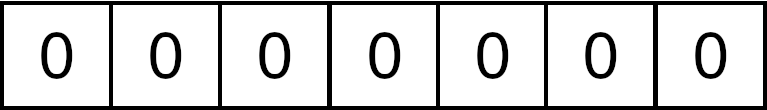
\includegraphics[scale=0.9]{figures/initial-bloom.png}
      \caption[Bloom Filter initial state]{Bloom Filter bit array initial state of \textit{m}=7}
      \label{fig:initial-bloom-filter}
    \end{center}
\end{figure}

% algorithm for insertion
\subsection*{Element Insertion}
Element insertion and query answering make use of \textit{k} hash functions, each mapping elements to a position in the bit array. Adding an element is done by determining which positions should be set to 1. To that end, the new element is fed into each hash function that maps the element to an array position. The resultant \textit{k} outputs are used as the \textit{k} positions of the array to be set to 1. Figure \ref{fig:insertion-bloom-filter} shows the insertion of element \textit{el} in the Bloom Filter, making use of three hash functions (\textit{k}=3), \textit{h\textsubscript{1}}, \textit{h\textsubscript{2}} and \textit{h\textsubscript{3}}. The outputs of the hash functions correspond to the array indexes to set to 1.

\begin{figure}[!htb]
    \begin{center}
      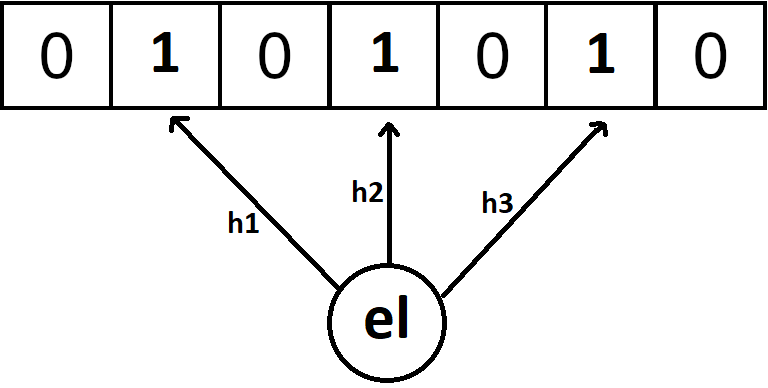
\includegraphics[scale=0.3]{figures/insert-bloom.png}
      \caption[Bloom Filter insertion]{Insertion of element \textit{el} into a Bloom Filter with \textit{m}=7 and \textit{k}=3}
      \label{fig:insertion-bloom-filter}
    \end{center}
\end{figure}

% algorithm for query
\subsection*{Membership Query}
Performing a membership query --- \textit{i.e.}, testing if an element \textit{el} is in the set --- is done by feeding \textit{el} into each one of the \textit{k} hash functions in order to get an array of positions. If \textit{el} was already in the set, all \textit{k} positions should be 1. If any position contains a 0 then the element is \textit{definitely not in set}, as shown in Figure \ref{fig:bloom-filter}. 

\begin{figure}[!htb]
    \begin{center}
      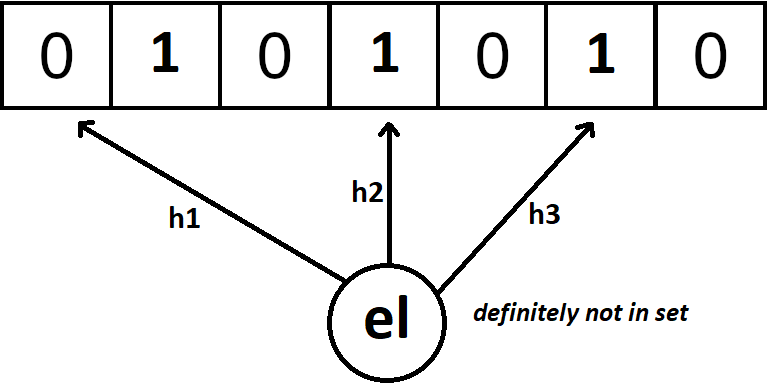
\includegraphics[scale=0.3]{figures/query-bloom.png}
      \caption[Bloom Filter membership query]{Bloom Filter membership test of element \textit{el}. Finding at least one ``0" indicates that it is not in the set.}
      \label{fig:bloom-filter}
    \end{center}
\end{figure}

If all positions are 1 then the element is said to be \textit{possibly in the set}. The reason a Bloom Filter does not provide 100\% certainty that \textit{el} is in the set in case of all positions being 1 is that hash functions may give the same position for two different elements. For example, hash functions \textit{h\textsubscript{1}}, \textit{h\textsubscript{2}} and \textit{h\textsubscript{3}} may map an element \textit{el1} to positions $[1,2,3]$ and an element \textit{el2} to positions $[4,5,6]$. This way, bits in positions $[1,2,3,4,5,6]$ are set to 1. When querying about the membership of a new element \textit{el3}, hash functions \textit{h\textsubscript{1}}, \textit{h\textsubscript{2}} and \textit{h\textsubscript{3}} may map it to positions $[1,3,5]$ as exemplified in Figure \ref{fig:bloom-filter-fp}. Since all of these positions are 1 because of the previous elements inserted, the Bloom Filter returns \textit{"possibly in set"} when in reality \textit{el3} was not in the set. This is considered a \textit{false positive}.

\begin{figure}[!htb]
    \begin{center}
      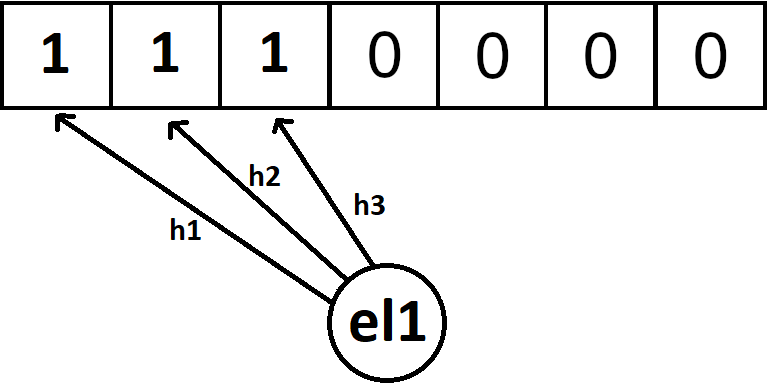
\includegraphics[scale=0.4]{figures/fp-bloom-1.png}
      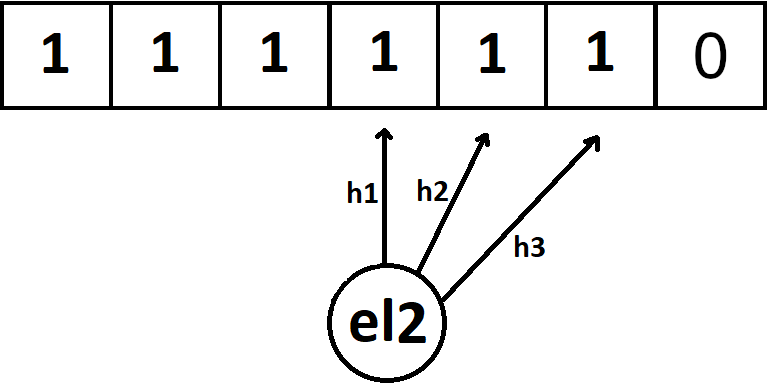
\includegraphics[scale=0.4]{figures/fp-bloom-2.png}
      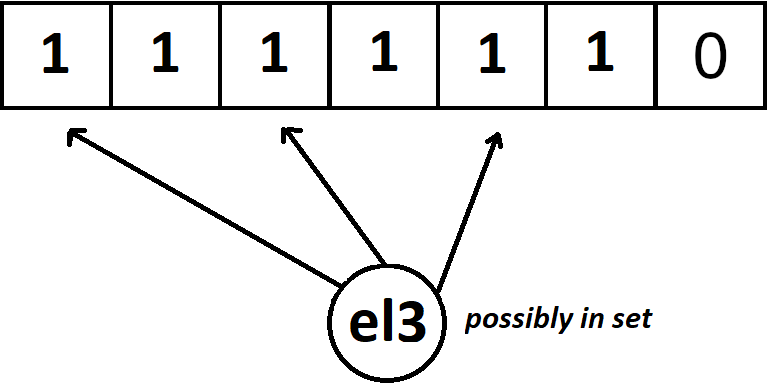
\includegraphics[scale=0.4]{figures/fp-bloom-3.png}
      \caption{Bloom Filter false positive}
      \label{fig:bloom-filter-fp}
    \end{center}
\end{figure}


\subsection*{False Positive rate}
% error bound related with parameters
The false-positive rate is a function of the bit array size \textit{m}, the number of hash functions \textit{k} and the number of elements in the set \textit{n}. It is assumed that the hash functions produce an independent and random index value for each element. 

Mullin presents an analysis of the Bloom Filter in \cite{Mullin-Bloom-Analysis} where he details the false positive rate formula. The probability of one arbitrary bit being set to 1 is:
\begin{equation}
    \frac{1}{m}
\end{equation}
because there are \textit{m} bits. Likewise, the probability of one bit not being set to 1 is
\begin{equation}
    1-\frac{1}{m}
\end{equation}

Mullin states the probability that an arbitrary bit is not set to 1 after one element insertion and corresponding \textit{k} bit updates is:
\begin{equation}
    (1-\frac{1}{m})^\textit{k}
\end{equation}

For \textit{n} insertions, the probability a bit is not set to 1 is:
\begin{equation}
    (1-\frac{1}{m})^\textit{kn}
\end{equation}

Therefore, the probability that an arbitrary bit is set to 1 after \textit{n} insertions is:
\begin{equation}
    1-(1-\frac{1}{m})^\textit{kn}
\end{equation}

Hence, the probability of false positive of a membership query for a new element for \textit{k} hash functions is given by
\begin{equation}
    (1-(1-\frac{1}{m})^\textit{kn})^\textit{k}
\end{equation}

Finally, this false positive rate can be approximated by 
\begin{equation}
    (1-e^\textit{-kn/m})^\textit{k}
\end{equation}


\subsection*{Optimal number of hash functions}
We want to choose the number of hash functions \textit{k} in order to minimize the false positive rate. In order to do so, we must first allocate \textit{m} bits for the Bloom Filter, choosing \textit{m} based on available memory. The value of \textit{k} that minimizes the false positive rate is either of the nearest integers given by:
\begin{equation}
    \frac{m}{n}ln(2)
\end{equation}

\subsection*{Time complexity analysis}
Considering a Bloom Filter with \textit{m} bits and \textit{k} hash functions, insertion has \textit{O(k)} time complexity because all there is to do is run the input through all of the \textit{k} hash functions and set the bits in the given positions to 1. Similarly, query answering has \textit{O(k)} time complexity because it needs only to run the input through the \textit{k} hash functions and check if all bits are set to 1. If so, it returns \textit{possibly in set}. Otherwise it returns \textit{definitely not in set}. 

Note that the time complexity does not at all depend on the number of elements processed by the Bloom Filter and that \textit{k} will be a rather small constant. Hence, the Bloom Filter is said to have constant time complexity.

\subsection*{Space complexity analysis}
Considering a Bloom Filter with \textit{m} bits, the space required is simply the array of \textit{m} bits, thus \textit{O(m)} space complexity. Similarly to the time complexity analysis, we point out that \textit{m} will be constant and that each of the array elements occupies 1 bit. Thus the Bloom Filter has a constant space complexity.

\subsection*{Applicability to our Hypothesis}
Bloom Filters exhibit constant space and time complexity making them possible methods to test our hypothesis. Their false positive rate is tolerable in most scenarios and can be controlled by tweaking the values of \textit{m} and \textit{k}. However, we need to evict old events, and for that reason, Bloom Filters are of no use to us.

\subsection{Item Frequency and the Count-Min Sketch}
% approx aggregation to compute
The Count-Min Sketch (CMS) uses two principles from the discussed Bloom Filters in Section \ref{sec:bloom}. First, Bloom Filters show that precision can be sacrificed to achieve space savings. Second, they are very similar at a technical level.

A Count–Min Sketch \cite{Cormode-CMS} is an approximate aggregator that estimates the frequency of each element in the dataset. It is named after the two basic operations used to provide the estimate: counting (\textit{count}) and computing the minimum (\textit{min}).

% data structures
\subsection*{Data structure}
A CMS is represented by a two-dimensional array (or matrix) with width \textit{w} and depth \textit{d}. A CMS will make use of \textit{d} hash functions, each associated with one row of the matrix. Each hash function will map elements to a position between 1 and \textit{w}, the column of the two-dimensional array. Initially, all of the matrix positions are 0. Figure \ref{fig:initial-cms} represents the two-dimensional array used by the CMS and corresponding dimensions in its initial state. 

\begin{figure}[!htb]
    \begin{center}
      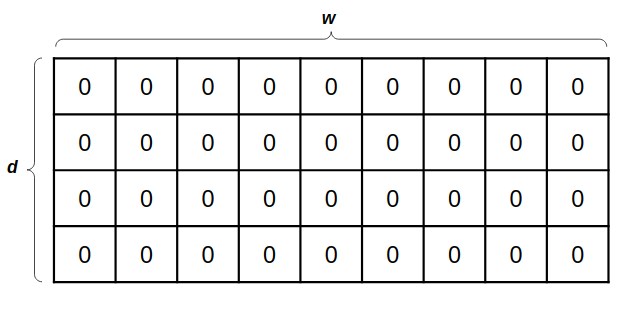
\includegraphics[scale=0.5]{figures/initial-cms.png}
      \caption[Count-Min Sketch initial state]{Count-Min Sketch matrix initial state of \textit{d}=4 and \textit{w}=9}
      \label{fig:initial-cms}
    \end{center}
\end{figure}

% algorithm for insertion
\subsection*{Element Insertion}
When adding an element, for each row \textit{i} of the \textit{d} rows in the matrix, we hash the element using that row's hash function to obtain the result $j$. Lastly, for all obtained pairs of \textit{i} and \textit{j}, increment matrix cells \textit{(i, j)} value by 1, as seen in Figure \ref{fig:cms}. If elements have different weights these can be added instead of incrementing one unit.

\begin{figure}[!htb]
    \begin{center}
      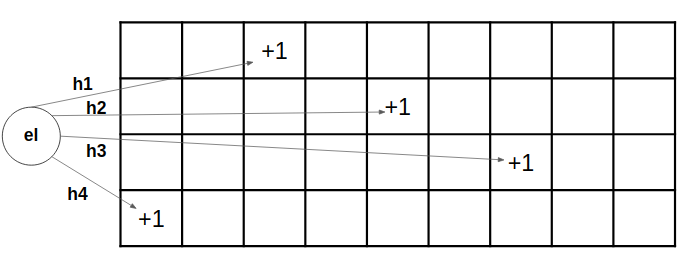
\includegraphics[scale=0.5]{figures/insertion-cms.png}
      \caption[Count-Min Sketch insertion]{CMS mapping element \textit{el} using \textit{d}=4 hash functions to determine the column position for each row and increment it.}
      \label{fig:cms}
    \end{center}
\end{figure}

% algorithm for query
\subsection*{Frequency Query}
Retrieving the minimum frequency of an element \textit{el} can be done by taking the minimum value of all row counts for \textit{el}. Mathematically, the frequency estimate is the minimum value of the set of all row values, for each row \textit{i} of the total \textit{d} rows, given by:
\[ min \{matrix[i][\textit{h\textsubscript{i}}(el)]\} \]

Figure \ref{fig:query-cms} illustrates this procedure, where the result of the query "What is the frequency of \textit{el}?" returns "2".
   
\begin{figure}[!htb]
    \begin{center}
      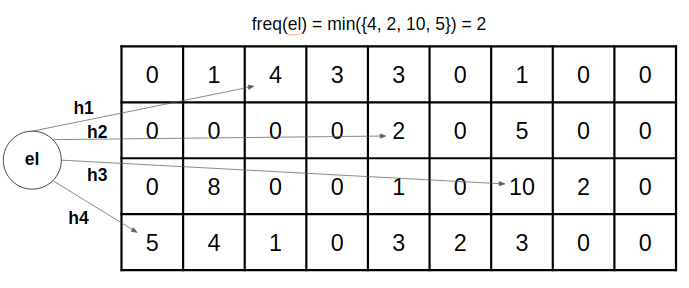
\includegraphics[scale=0.5]{figures/query-cms.png}
      \caption[Count-Min Sketch frequency query]{Count-Min Sketch frequency query of element \textit{el}}
      \label{fig:query-cms}
    \end{center}
\end{figure}

% error bound related with parameters
\subsection*{Optimal number of hash functions} 
For an element \textit{el}, each row will have one position incremented by \textit{el}'s true frequency. However, multiple elements may be mapped to the same position within a row, thus overlapping their frequencies. Hence, for an element \textit{el}, the CMS provides a frequency estimate that is greater or equal to the true frequency of \textit{el} in the set.

The number of hash functions \textit{d} to be used depends on the desired error probability. To achieve an error probability $\delta$, \textit{d} is given by the following expression:
\begin{equation}
    d = \lceil ln \frac{1}{\delta} \rceil
\end{equation}
For example, to achieve an error $\delta$ = 1\%, \textit{d} = 5 hash functions are necessary.

\subsection*{Time complexity analysis}
When adding an element, the Count-Min Sketch loops through each row and applies a constant in time hash function, updating the value of the target cell. Hence, insertion loops through \textit{d} rows and has time complexity of \textit{O(d)}. Similarly, querying the frequency of an element \textit{el} consists of computing the minimum of all row values. Since both insertion and query have constant time complexity, the CMS is constant in time.

\subsection*{Space complexity analysis}
The Count-Min Sketch relies on a two-dimensional matrix as its only data structure. The memory used will correspond to the \textit{wd} counts, hence \textit{O(wd)} space complexity. Since both \textit{w} and \textit{d} are constants, the CMS has constant space complexity.

\subsection*{Applicability to our Hypothesis}
Count-Min Sketches are constant in both time and space. Similarly to Bloom Filters, this makes them ideal candidates for our solution. 

\subsection{Cardinality Estimation and the HyperLogLog} \label{sec:hyper-log-log}

A set of probabilistic counting algorithms is introduced by Flajolet \emph{et al.} in \cite{Flajolet-PCA} to estimate the number of distinct elements of a set --- also known as the cardinality of the set. These techniques are based on \textit{"bit-pattern observables"} in the binary representation of the hashed values. Bit-pattern observables are defined by the authors as \textit{"patterns of bits occurring at the beginning of the (binary) S-values"}, with \textit{S} as the target set.

Later on, the authors propose the LogLog algorithm \cite{Flajolet-LogLog}. In LogLog, the bit-pattern observable recorded for each item is the position of the leftmost 1-bit, denoted as \textit{P}. The authors claim it is related to the total number of distinct elements in the dataset in that it is \textit{"more or less a likely indication that the cardinality of S is at least $2^P$"}.


\subsection*{HyperLogLog}
A couple of years later, the same authors propose HyperLogLog (HLL) \cite{Flajolet-HLL}, an approximate aggregator to compute the cardinality of a set. 

HLL uses the same bit-pattern observable as LogLog --- \textit{P}, the position of the leftmost 1-bit. With LogLog, the authors realize that storing only one observation produces extremely inaccurate predictions due to the high variability of a single value. The proposed solution is to apply \textit{stochastic averaging}. As the authors state, stochastic averaging \textit{"consists in emulating the effect of m experiments"}. Effectively speaking, the authors propose dividing the input stream into \textit{m} substreams or buckets, maintaining one observable per bucket and computing \textit{P} as an average of all bucket values (stochastic averaging).

\subsection*{Data Structure}
HyperLogLog (HLL) maintains \textit{m} bit-pattern observables, each being the leftmost 1-bit position, \textit{P}. Since each position is a single integer, HLL maintains \textit{m} integer counters, as seen in Figure \ref{fig:hll-ds}. Each of these counters holds the maximum value for the bit-pattern observable seen so far. The first bit is assumed to be in position "1" and all counters begin with "0".

\begin{figure}[!htb]
    \begin{center}
       \hspace{0.5in}
      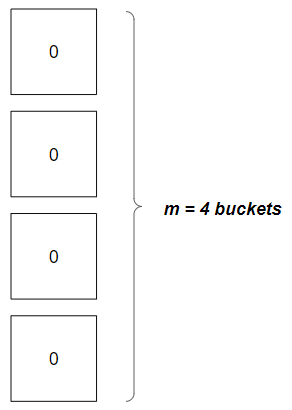
\includegraphics[scale=0.6]{figures/hll-ds.png}
      \caption[HyperLogLog initial state]{HyperLogLog with \textit{m}=4 observable buckets}
      \label{fig:hll-ds}
    \end{center}
\end{figure}


\subsection*{Element Insertion}
In HyperLogLog, new elements are hashed into a binary string. The first \textit{n} bits of the hashed representation will map to one of the $m=2^n$ buckets. Effectively speaking, the first \textit{n} bits work as a \textit{bucket ID}. The bit-pattern observable \textit{P} --- the position of the leftmost 1-bit --- is counted from the binary string discarding the first \textit{n} bits. The observable \textit{P} is stored in the pre-determined bucket if it is greater than the value the bucket contains. 

Figure \ref{fig:hll-insert} demonstrates such procedure for a new element \textit{el}. The hash representation of \textit{el}, using $n=2$ bits, maps to bucket \textit{10}. Discarding the first $n=2$ bits and counting from 1, the position of the leftmost 1-bit is $P=4$. The previous value of bucket \textit{10} was 0 and because $P=4$ is greater than 0 the bucket value is updated.


\begin{figure}[!htb]
    \begin{center}
      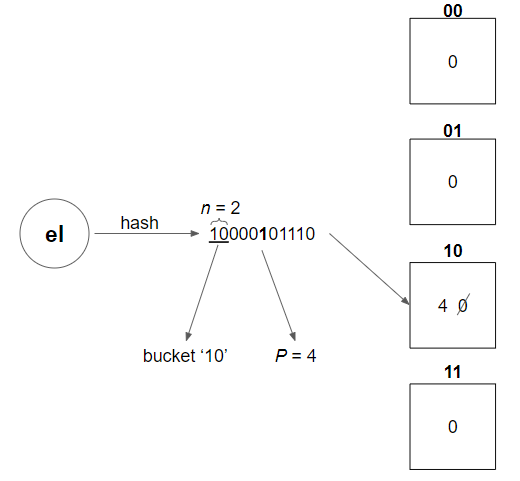
\includegraphics[scale=0.8]{figures/hll-insertion.png}
      \caption[HyperLogLog insertion]{HyperLogLog \textit{el} insertion with \textit{m}=4 and \textit{n}=2 bits}
      \label{fig:hll-insert}
    \end{center}
\end{figure}

\subsection*{Cardinality Query}
The cardinality of the set is estimated to be $2^\textit{P}$ where the bit-pattern observable \textit{P} is the position of the leftmost 1-bit. As discussed, HyperLogLog (HLL) differentiates from LogLog in that it applies a stochastic averaging process. Hence, the value of \textit{P} will be the harmonic mean of all \textit{m} buckets.


\subsection*{Time complexity analysis}
Adding an item is tantamount to hashing it, determining the corresponding bucket based on the first \textit{n} bits, counting the leftmost 1-bit position and updating the bucket value if need be. Estimating the cardinality of the set amounts to finding the maximum value \textit{P} between all buckets and computing $2^P$. Hence, both inserting a new element and estimating the cardinality of the set take constant time.

\subsection*{Space complexity analysis}
Quoting Flajolet \emph{et al.} about the memory consumption and error in the approximations obtained in their experiments in the original HyperLogLog paper \cite{Flajolet-HLL}: 
\say{cardinalities till values over N = $10^9$ can be estimated with a typical accuracy of 2\% using 1.5kB (kilobyte) of storage.}

HyperLogLog uses \textit{m} buckets that store a single integer value, thus the space complexity is \textit{O(m)} where \textit{m} is a rather small constant. Hence, HyperLogLog has constant space complexity.

\subsection*{Applicability to our Hypothesis}
Similar to the previously studied approximate aggregators, HyperLogLog (HLL) has constant space and time complexity and provides an estimate of a set's cardinality. Hence, HLLs are considered valuable aggregators for our thesis.

\section{Sliding Window Aggregations with Probabilistic Data Structures} \label{sec:sliding-pds}
In Section \ref{sec:pds} we presented a set of probabilistic data structures constant in time and space. These structures aggregate an endless stream of data. However, when working with sliding windows there is the need not only to insert new events but to evict old ones. The probabilistic data structures described until now can aggregate new incoming data but do not address the type of temporality needed for sliding windows --- \textit{i.e.}, the ability to expire old elements from the aggregated state.

The probabilistic data structures studied can be implemented under generic sliding window aggregation algorithms like Recalculate-From-Scratch or DABA. However, doing so means we lose the main advantage of using these approximate aggregators: the constant space complexity. For example, cardinality estimation of a sliding window can be done employing the HyperLogLog heuristic of estimating cardinality as $2^\textit{p}$, with \textit{p} as the maximum position seen for the leftmost 1-bit, using DABA \ref{sec:daba} for the computation of \textit{p} per sliding window. With this approach, despite computing the aggregation state in constant time, we have a linear in window size space complexity solution. Thus, in this section, we explore sliding window implementations of the previously discussed probabilistic data structures that keep the space and time complexity at the very least logarithmic.

%\subsection{Sliding Bloom Filter}
%\subsection*{Data Structure}
%\subsection*{Element Insertion}
%\subsection*{Element Eviction}
%\subsection*{Time complexity analysis}
%\subsection*{Space complexity analysis}
%\subsection*{Applicability to our Hypothesis}

%\subsection{Sliding Count-Min Sketch}
%\subsection*{Data Structure}
%\subsection*{Element Insertion}
%\subsection*{Element Eviction}
%\subsection*{Time complexity analysis}
%\subsection*{Space complexity analysis}
%\subsection*{Applicability to our Hypothesis}


\subsection{Sliding HyperLogLog}

The HyperLogLog (HLL) aggregator presented in Section \ref{sec:hyper-log-log} will only be useful to us if it can be implemented efficiently in a sliding window fashion. The HLL aggregator estimates the set's cardinality assuming it is close to $2^\textit{p}$, where \textit{p} is the maximum position seen for the leftmost 1-bit in the binary values of all of the set items' hashes. In practice, all the aggregator has to compute is \textit{p}, the maximum value of all observables. Stochastic averaging is applied by emulating the effects of \textit{m} experiments using \textit{m} buckets to store \textit{m} bit-pattern observables. 


\subsubsection{Sliding HyperLogLog using Lists of Future Possible Maxima} \label{sec:hll-lfpm}

The work of Chabchoub \emph{et al.} adapts the original HLL aggregator from Flajolet \emph{et al.} to work under a sliding window framework  \cite{Chabchoub-Sliding-HLL}.
The main idea behind this implementation is to replace every HLL counter with a \textit{List of Future Possible Maxima (LFPM)}.

\subsubsection*{Data Structure}

The adaptation of the original HLL to work under a sliding window scenario requires the storage of additional information. The original HLL maintained \textit{m} integer counters, each storing the maximum for the leftmost 1-bit position of the analyzed binary strings.  The counter held the maximum value for all the seen binary strings so far but there was no way to expire old items. To allow eviction, the proposed data structure is very similar to the original \textit{m} integer counters but keeps a list of values per bucket and associates a timestamp to each. 

The stochastic averaging process of HLL remains unchanged: incoming items are hashed and distributed across \textit{m} buckets. However, the authors propose keeping a short list of \textit{packets} per bucket instead of a single integer count. A \textit{packet} is defined as a pair <\textit{t\textsubscript{i}, p\textsubscript{i}}> where \textit{t\textsubscript{i}} is the arrival timestamp of the packet and \textit{p\textsubscript{i}} the position of the leftmost 1-bit in the binary hash representation of the associated value. Packets are only kept in the list if they are possible maxima over future windows. Because of that, the authors name this list a ``List of Future Possible Maxima (LFPM)''.

\subsubsection*{Element Insertion \& Eviction}
Similarly to the original HLL, incoming elements are hashed and the first \textit{n} bits of the string are used to map the new element to one of the \textit{m} buckets. The first \textit{n} bits are then discarded and the bit-pattern observable \textit{p} is computed from the remaining string. 

Since each bucket now holds a LFPM instead of a single integer, the procedure for bucket update is different. Upon insertion of an element \textit{k}, a packet $<t_k, p_k>$ is created with t\textsubscript{k} as the timestamp of arrival of the new element \textit{k} and p\textsubscript{k} as the position of the leftmost 1-bit position of \textit{k}'s binary representation. Given the new packet <t\textsubscript{k}, p\textsubscript{k}>, the authors propose the following LFPM update method, that checks for and evicts old packets at each insertion:

\begin{itemize}
    \item Delete \textit{old packets}: packets that do not belong in the window anymore --- \textit{i.e.}, packets <t\textsubscript{i}, p\textsubscript{i}> with t\textsubscript{i} $\leq$ t\textsubscript{k} - WindowSize 
    
    \item Delete less or equally valued packets: packets that will never be a maximum --- \textit{i.e.}, packets <t\textsubscript{i}, p\textsubscript{i}> with p\textsubscript{i} $\leq$ p\textsubscript{k}
    
    \item Add the new packet <t\textsubscript{k}, p\textsubscript{k}>
\end{itemize}


\subsubsection*{Sliding Window Cardinality Query} 

Estimation of cardinality is done similarly to the original HLL cardinality estimation algorithm. To estimate the cardinality at a timestamp \textit{t}, from all \textit{m} buckets and all \textit{m} lists, select packets that are in the window --- \textit{i.e.}, packets <t\textsubscript{i}, p\textsubscript{i}> where t\textsubscript{i} > \textit{t} - WindowSize. This filtering is necessary since the proposed algorithm evicts old packets only at element insertion and at the time of the query some packets may no longer belong to the window. Next, from the filtered set of packets, for each bucket and its list, compute the maximum p\textsubscript{i} value. In the end, compute the harmonic mean between all values, just like the original HLL. The result will be the averaged bit-pattern observable value \textit{p} and the cardinality is estimated to be $2^\textit{p}$.

\subsubsection*{Time complexity analysis}
When performing insertions or evictions, the algorithm requires scanning through the Lists of Future Possible Maxima (LFPMs) to delete old packets or packets that will never be window maxima. Similarly, we need to scan the lists when estimating the cardinality to filter for packets within our window. Denote \textit{L\textsubscript{n}} as the mean size in packets for each LFPM. There are \textit{m} buckets, each with a list. To scan through all lists we need to analyze \textit{m L\textsubscript{n}} elements. 

The authors prove that \textit{L\textsubscript{n}} has an upper bound of \textit{ln(n/m)}, with \textit{n} as the cardinality of the set and \textit{m} as the number of buckets used. Hence, in the worst-case scenario, we need to analyze \textit{m ln(n/m)} elements. This means that a Sliding HLL implementation using Lists of Future Possible Maxima has \textit{O(ln(n))} time complexity, given the number of buckets \textit{m} is constant.

\subsubsection*{Space complexity analysis}
The memory used in the Sliding HLL aggregator implemented with Lists of Future Possible Maxima (LFPMs) amounts to the total size of the \textit{m} lists. Assuming 4 byte timestamps and 1 byte bit-pattern observables for each packet, the aggregator uses \textit{(4+1) L\textsubscript{n} m} bytes. 

The lists are dynamic thus they shrink and grow at runtime. However, \textit{ln(n/m)} was proved to be an upper bound for \textit{L\textsubscript{n}}. Hence, this sliding implementation of the HLL aggregator consumes up to \textit{(4+1) ln(n/m) m} bytes of memory. Considering that the number of buckets \textit{m} is constant, the space complexity of a Sliding HLL implementation with LFPM is \textit{O(ln(n))}.

The authors claim that the proposed sliding version remains as accurate as of the original HLL aggregator. With an additional memory of only 35kB, it is possible to estimate the number of distinct elements in the set with a standard error of 3\% in the presence of up to a million distinct elements.

\subsubsection*{Applicability to our Hypothesis}
Implementing a Sliding HLL using Lists of Future Possible Maxima (LFPMs) shows logarithmic time and space complexity while providing estimates with the same accuracy as the original HLL approximate aggregator. However, the memory consumption is dynamic due to the variable size of the lists. 

Despite the fact memory consumption dynamically changes during runtime, this is a valid approach to test our Hypothesis due to the worst-case scenario being a logarithmic space complexity. However, in Section \ref{sec:hll-drv} we analyze an implementation that is not dynamic in memory during runtime making it a preferred approach.


\subsubsection{Sliding HyperLogLog using Distance Recorder Vectors} \label{sec:hll-drv}

In Section \ref{sec:hll-lfpm} we have analyzed a Sliding HLL implementation where each of the \textit{m} buckets holds a list of values (LFPM) instead of a single integer count. However, the LFPM structure is dynamic and its size varies at runtime. 

The approach proposed by Xu uses a smaller amount of memory that does not change at runtime \cite{Xu-hll-sliding-drv}. The author proposes a special counter: a \textit{Distance Recorder Vector (DRV)}. 

\subsubsection*{Data Structure}
Much like the original HLL and the LFPM Sliding implementation, the Distance Recorder Vector (DRV) approach uses \textit{m} buckets. However, instead of integer counts or lists, each of the buckets stores a DRV. 

A DRV is composed by \textit{$\lceil ln(n/m) \rceil$} records, with \textit{n} as the cardinality of the set. Notice that \textit{n/m} is the average number of distinct elements each bucket \textit{m} is expected to process and that a binary string of size \textit{$\lceil ln(n/m) \rceil$} can represent \textit{n/m} distinct elements. Also recall that the bit-pattern observable \textit{p} used by the HLL is the position of the leftmost 1-bit. In a binary string of size \textit{$\lceil ln(n/m) \rceil$}, \textit{p} will range from 1 to \textit{$\lceil ln(n/m) \rceil$}. The DRV is indexed exactly this way, from 1 to \textit{$\lceil ln(n/m) \rceil$}, and each bit-pattern observable \textit{p} will be used as an index in this vector of records. Essentially, each \textit{p} will have an associated record in a DRV of a bucket.

Initially, all records in the DRV will be set to be infinity or a very large number.

\subsubsection*{Element Insertion}
When an element is inserted, the same procedure as in the original HLL is followed: the element is hashed and \textit{p} is computed from the hashed binary representation. Let us denote the bit-pattern observable of the new element as \textit{p\textsubscript{new}}. For the DRV of that bucket, we increment the value of all records by one. Next, we set position \textit{p\textsubscript{new}} in the DRV to 0 --- \textit{i.e.}, $\textrm{DRV}[p_{new}] = 0$.


\subsubsection*{Sliding Window Cardinality Query} 
This method does not perform element eviction. Instead, the query algorithm assumes that some records in DVR's entries might be expired. 

To estimate the sliding window cardinality is to find the value \textit{p}. To find the value \textit{p} for a bucket, we scan the DRV of that bucket backward. For that, we start at the last element --- positioned at \textit{$\lceil ln(n/m) \rceil$} --- and scan towards the head of the vector. For each record, we check if it is active in the current window. To do so, we check if its value is less than the size of the window. If it is, the record is active. Otherwise, the record is inactive.

If the record is inactive we continue scanning backward. If the record is active, then the position or index currently being scanned is the value of \textit{p} for that bucket. If all records are inactive, the bit-pattern observable \textit{p} is 0.

Stochastic averaging is done just like in the original HLL: compute the harmonic mean of all \textit{p\textsubscript{m}} values from all \textit{m} buckets. The cardinality of the sliding window is then estimated to be $2^\textit{p}$.

\subsubsection*{Time complexity analysis}
When inserting an element, determining its bucket, hashing the element and computing \textit{p} is done in constant time. However, all the  \textit{$\lceil ln(n/m) \rceil$} records must have their value increased by one and this means iterating over the DRV. Setting the element of the DRV indexed by \textit{p} to 0 is done in constant time as well. 

Estimating cardinality is done by scanning the DRV backward until an active record is found. In the worst-case scenario, this means scanning all \textit{$\lceil ln(n/m) \rceil$} records.

Both inserting an element and estimating sliding window cardinality require a scan through \textit{$\lceil ln(n/m) \rceil$} records. This gives us a time complexity of \textit{O(\textit{ln(n)})}, if the number of buckets \textit{m} is constant. 

\subsubsection*{Space complexity analysis}
This approach still uses \textit{m} buckets but each one contains a Distance Recorder Vector (DRV). A DRV is a vector of \textit{$\lceil ln(n/m) \rceil$} elements. Hence, \textit{$m \lceil ln(n/m) \rceil$} elements must be kept in memory, giving us a space complexity of \textit{O(ln(n))} with \textit{n} as the cardinality of the set.

\subsubsection*{Applicability to our Hypothesis}
Despite having the same time and space complexities, the Sliding HLL DRV approach uses a smaller amount of memory that does not change during runtime, while the LFPM requires heap resizing because the lists dynamically shrink and grow. Hence, the DRV approach is a better fit to integrate our lightweight real-time solution, if we need to perform cardinality estimation.


\section{Summary}
In this chapter, we presented state of the art outlier detection methods and classified them according to Blázquez-García \emph{et al.} taxonomy \cite{Blazquez-Garcia-Review-Anomaly-Detection}. Additionally, we presented sliding window aggregation algorithms, probabilistic data structures and their respective sliding window implementations, with the intent of researching how to incrementally maintain an aggregation in a streaming environment.

In Section \ref{sec:outliers}, we reviewed outlier detection algorithms. However, we found most of them inapplicable in our scenario, because they were resource-intensive (both time and memory-wise), provided no measure of how divergent an outlier was or because they evolved their reference period.

In Section \ref{sec:sota-swag-algs}, we presented sliding window aggregation algorithms that we intended on using to compute our aggregations. However, their time or memory complexities did not meet our sub-linear requirements.

We then discussed probabilistic data structures (Section \ref{sec:pds}) and their sliding window implementations (Section \ref{sec:sliding-pds}). Despite being efficient, both time and memory-wise, each probabilistic data structure allows for one type of aggregation, and none of them happened to be of particular use to us.

In the next chapter, we formally define the problem we aim to solve and the issues with current state of the art solutions. Then, we formulate our proposal along with the assumptions we make when approaching this problem. Finally, we pose some research questions we aim to answer by the end of this thesis.
